\section{\label{sec:level1}Observation and Analysis}
    \subsection{Magnetoresistance}
    
        \subsubsection{I=198.5mV}
            The magnetoresistance data for $I=198.5mA$ is shown in \hyperref[tab:mag1]{Table 1} and the graph of $\frac{\Delta R}{R}$ vs $H$ is shown in \hyperref[fig:graph1]{Figure.1}. The graph of $\log (\frac{\Delta R}{R})$  vs $\log(H)$ is shown in \hyperref[fig:graph2]{Figure.2}.
            \begin{table}[h]
	\centering
	\begin{tabular}{|c|c|c|c|}
	\hline
	\textbf{\begin{tabular}[c]{@{}c@{}}Angle\\ $(\theta)$\end{tabular}} & \textbf{Time (s)} & \textbf{Counts} & \textbf{\begin{tabular}[c]{@{}c@{}}Counts per\\ second $N(\theta)$\end{tabular}} \\ \hline
	\multirow{5}{*}{25} & \multirow{5}{*}{600} & 133 & \multirow{5}{*}{0.225} \\ \cline{3-3}
	 &  & 140 &  \\ \cline{3-3}
	 &  & 127 &  \\ \cline{3-3}
	 &  & 137 &  \\ \cline{3-3}
	 &  & 138 &  \\ \hline
	\multirow{5}{*}{20} & \multirow{5}{*}{200} & 164 & \multirow{5}{*}{0.940} \\ \cline{3-3}
	 &  & 198 &  \\ \cline{3-3}
	 &  & 186 &  \\ \cline{3-3}
	 &  & 195 &  \\ \cline{3-3}
	 &  & 197 &  \\ \hline
	\multirow{5}{*}{15} & \multirow{5}{*}{100} & 311 & \multirow{5}{*}{2.929} \\ \cline{3-3}
	 &  & 276 &  \\ \cline{3-3}
	 &  & 277 &  \\ \cline{3-3}
	 &  & 311 &  \\ \cline{3-3}
	 &  & 290 &  \\ \hline
	\multirow{5}{*}{10} & \multirow{5}{*}{100} & 1726 & \multirow{5}{*}{17.626} \\ \cline{3-3}
	 &  & 1811 &  \\ \cline{3-3}
	 &  & 1713 &  \\ \cline{3-3}
	 &  & 1754 &  \\ \cline{3-3}
	 &  & 1809 &  \\ \hline
	\multirow{5}{*}{5} & \multirow{5}{*}{100} & 2931 & \multirow{5}{*}{29.286} \\ \cline{3-3}
	 &  & 2938 &  \\ \cline{3-3}
	 &  & 2912 &  \\ \cline{3-3}
	 &  & 2931 &  \\ \cline{3-3}
	 &  & 2931 &  \\ \hline
	\multirow{5}{*}{-5} & \multirow{5}{*}{100} & 2934 & \multirow{5}{*}{29.343} \\ \cline{3-3}
	 &  & 2933 &  \\ \cline{3-3}
	 &  & 2935 &  \\ \cline{3-3}
	 &  & 2935 &  \\ \cline{3-3}
	 &  & 2935 &  \\ \hline
	\multirow{5}{*}{-10} & \multirow{5}{*}{100} & 1751 & \multirow{5}{*}{17.824} \\ \cline{3-3}
	 &  & 1778 &  \\ \cline{3-3}
	 &  & 1831 &  \\ \cline{3-3}
	 &  & 1787 &  \\ \cline{3-3}
	 &  & 1766 &  \\ \hline
	\multirow{5}{*}{-15} & \multirow{5}{*}{100} & 291 & \multirow{5}{*}{2.940} \\ \cline{3-3}
	 &  & 294 &  \\ \cline{3-3}
	 &  & 289 &  \\ \cline{3-3}
	 &  & 290 &  \\ \cline{3-3}
	 &  & 306 &  \\ \hline
	\multirow{5}{*}{-20} & \multirow{5}{*}{200} & 210 & \multirow{5}{*}{1.009} \\ \cline{3-3}
	 &  & 194 &  \\ \cline{3-3}
	 &  & 211 &  \\ \cline{3-3}
	 &  & 201 &  \\ \cline{3-3}
	 &  & 194 &  \\ \hline
	\multirow{5}{*}{-25} & \multirow{5}{*}{600} & 133 & \multirow{5}{*}{0.225} \\ \cline{3-3}
	 &  & 140 &  \\ \cline{3-3}
	 &  & 127 &  \\ \cline{3-3}
	 &  & 135 &  \\ \cline{3-3}
	 &  & 141 &  \\ \hline
	\end{tabular}
	\caption{Table for $N(\theta)$ for 5mm thick Gold foil}
	\label{tab:1}
\end{table}
            \begin{figure}[]
                \centering
                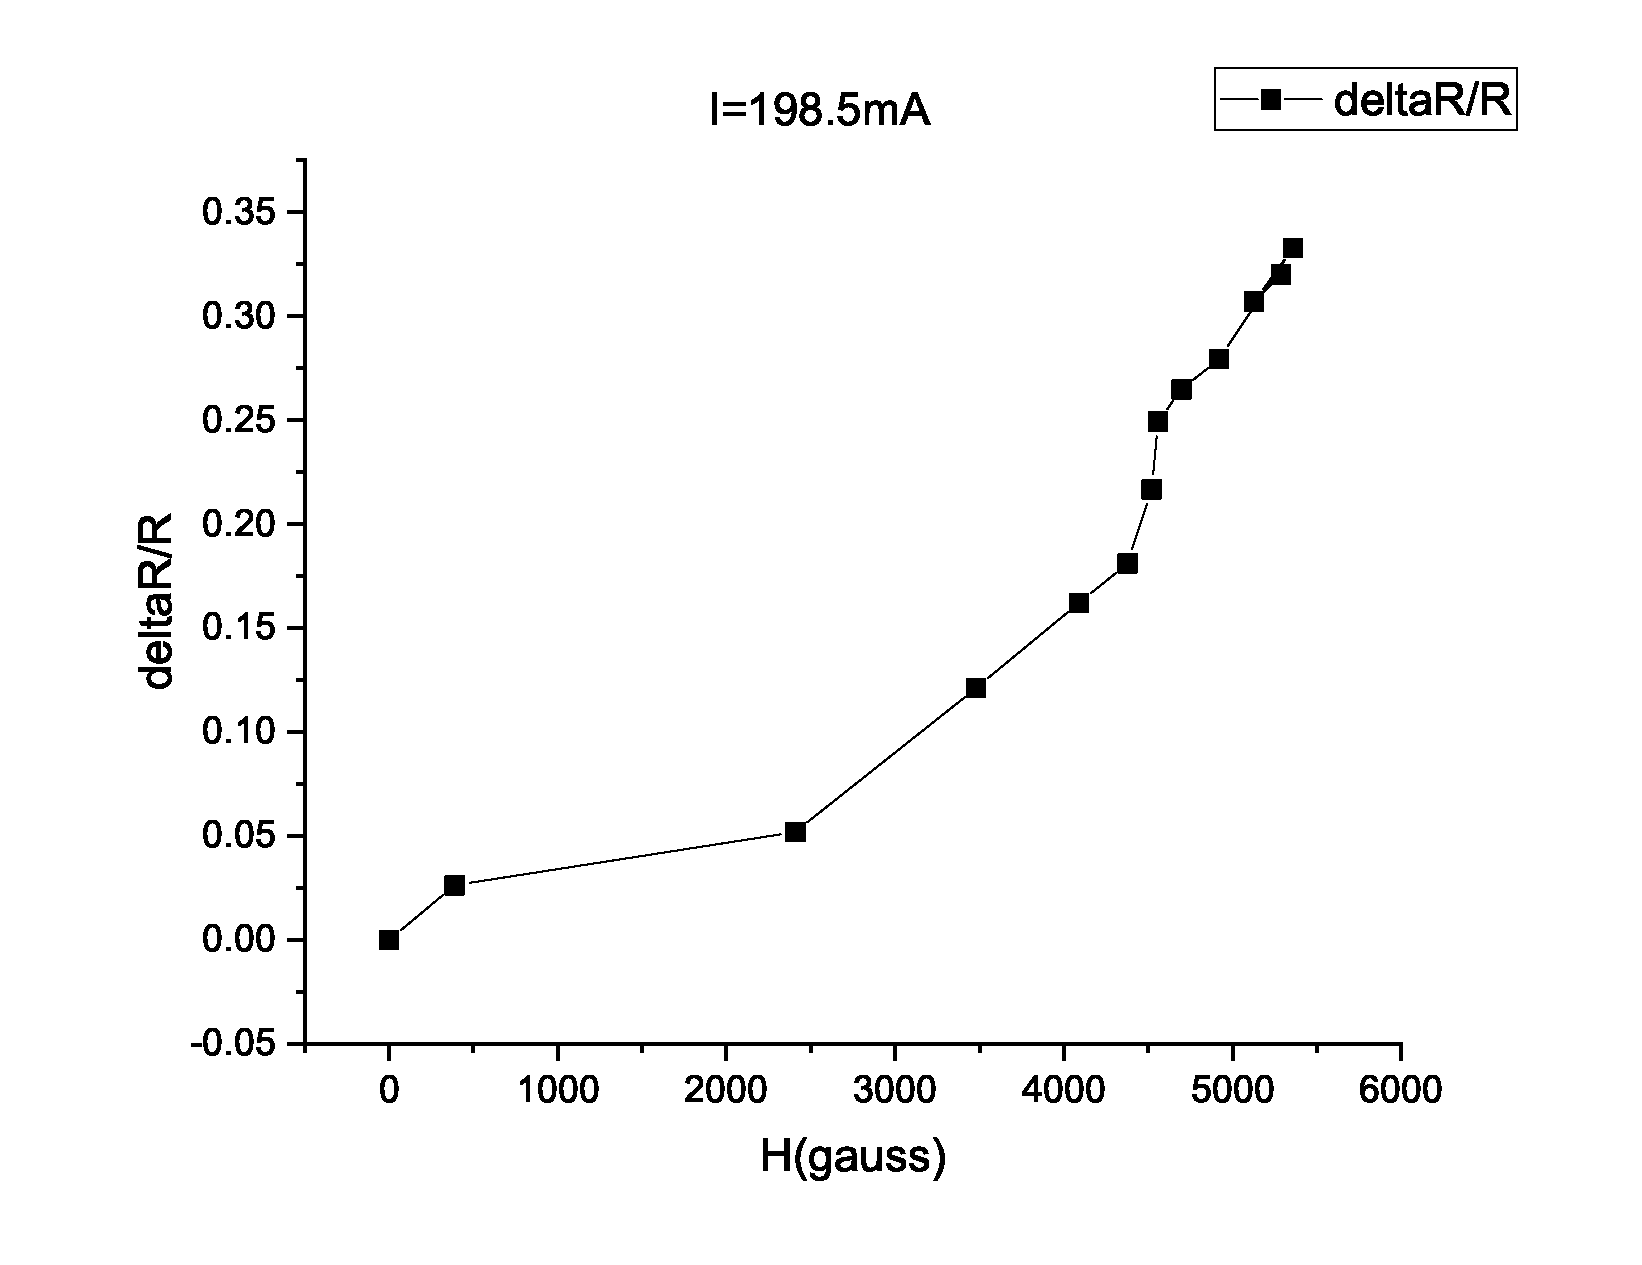
\includegraphics[width=0.95\columnwidth]{images/Graph1.eps}
                \caption{$\frac{\Delta R}{R}$ vs $H$}
                \label{fig:graph1}
            \end{figure}
            \begin{figure}[]
                \centering
                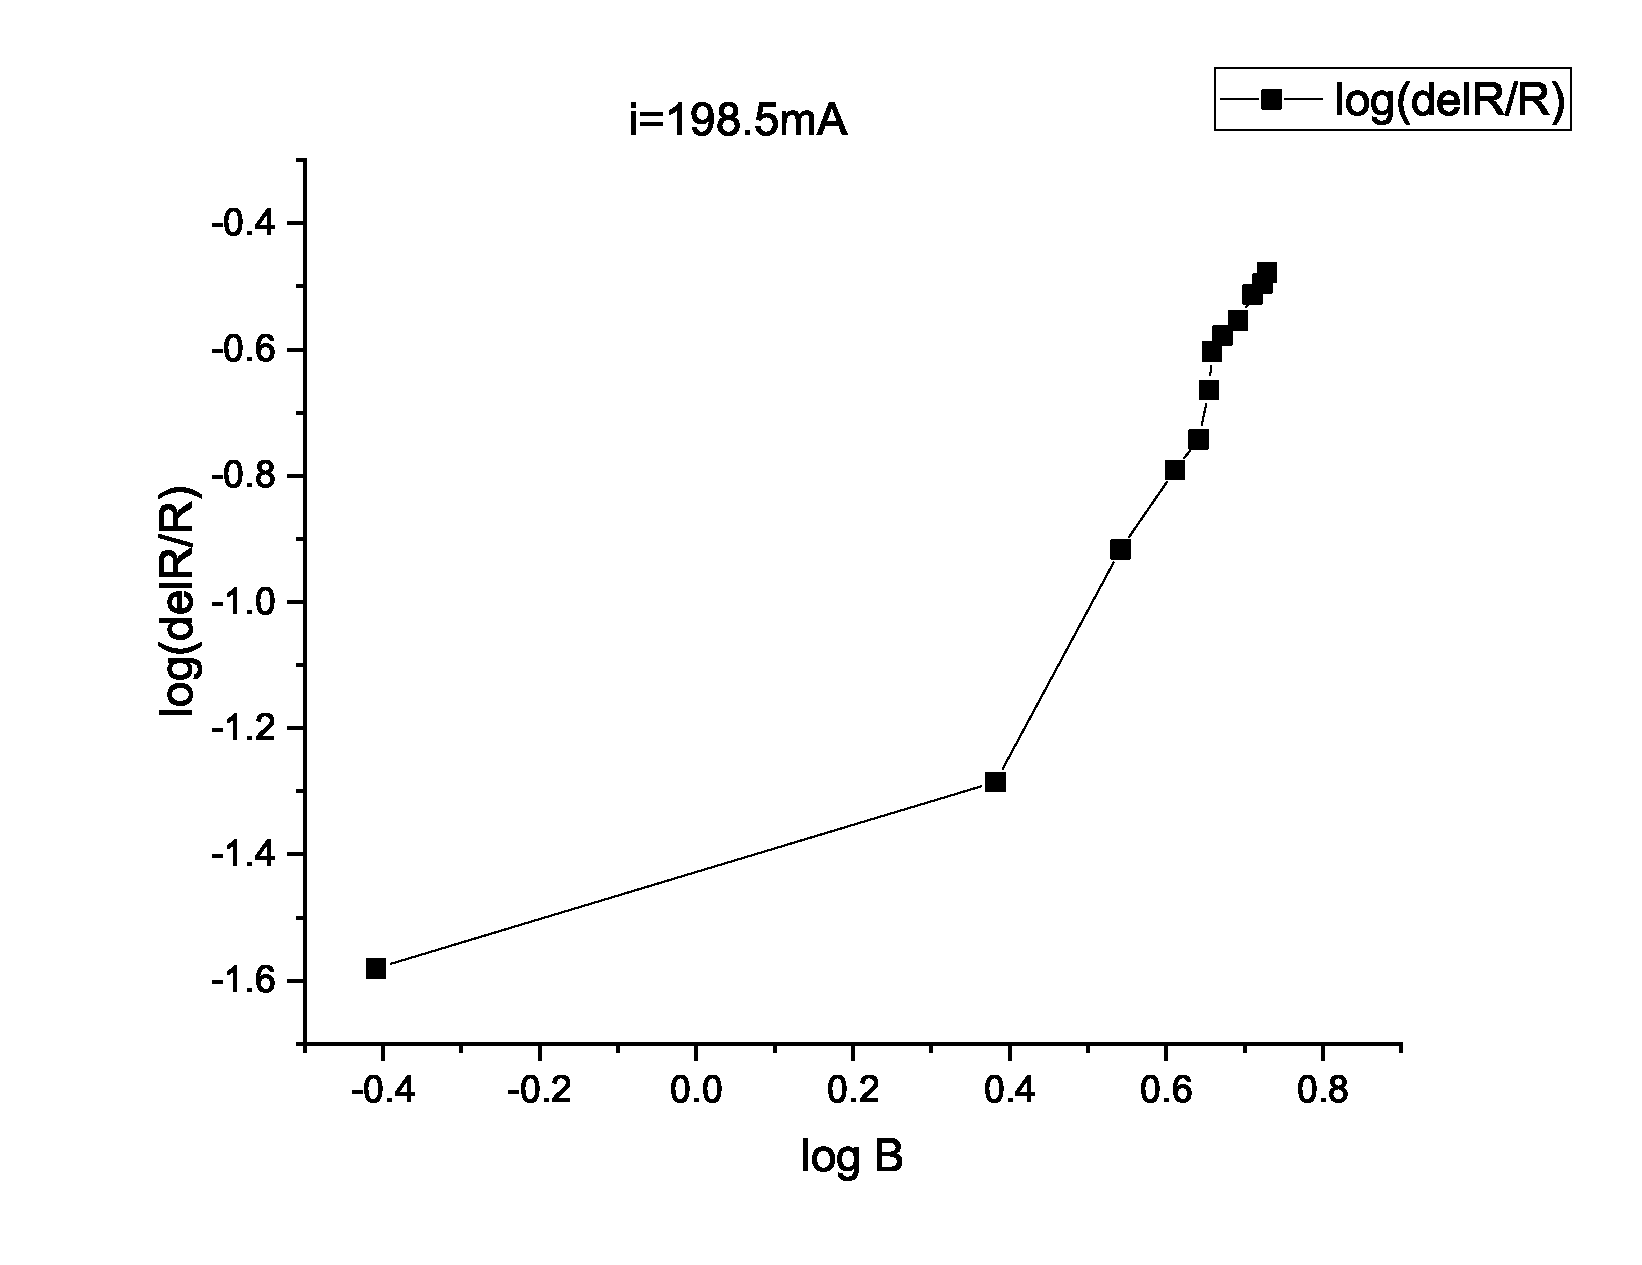
\includegraphics[width=0.95\columnwidth]{images/Graph2.eps}
                \caption{$\log (\frac{\Delta R}{R})$  vs $\log(H)$}
                \label{fig:graph2}
            \end{figure}


        \subsubsection{I=101.0mA}
            The magnetoresistance data for $I=101.0mA$ is shown in \hyperref[tab:mag2]{Table 2} and the graph of $\frac{\Delta R}{R}$ vs $H$ is shown in \hyperref[fig:graph3]{Figure.3}. The graph of $\log(\frac{\Delta R}{R})$ vs $H$ is shown in \hyperref[fig:graph4]{Figure.4}.
            \begin{table}[H]
    \centering
    \begin{tabular}{|c|c|c|c|}
        \hline
        $V_{DC}$ & $V_{DUT}$ & $V_{OUT}$ & $C_{DUT}$   \\ \hline
        0        & 0.074     & 0.459     & 127.837 \\
        0.1      & 0.109     & 0.451     &  85.276 \\
        0.2      & 0.232     & 0.447     &  39.709 \\
        0.3      & 0.299     & 0.438     &  30.191 \\
        0.4      & 0.389     & 0.432     &  22.888 \\
        0.5      & 0.463     & 0.432     &  19.230 \\
        0.6      & 0.564     & 0.426     &  15.567 \\
        0.7      & 0.662     & 0.420     &  13.075 \\
        0.8      & 0.760     & 0.435     &  11.796 \\
        0.9      & 0.846     & 0.430     &  10.475 \\
        1        & 0.941     & 0.426     &   9.330 \\
        1.1      & 1.058     & 0.427     &   8.318 \\
        1.2      & 1.174     & 0.422     &   7.408 \\
        1.3      & 1.267     & 0.418     &   6.799 \\
        1.4      & 1.357     & 0.416     &   6.318 \\
        1.5      & 1.464     & 0.412     &   5.800 \\
        1.6      & 1.559     & 0.409     &   5.406 \\ \hline
    \end{tabular}
    \caption{Data for light condition}
    \label{tab:2}
\end{table}
            \begin{figure}[]
                \centering
                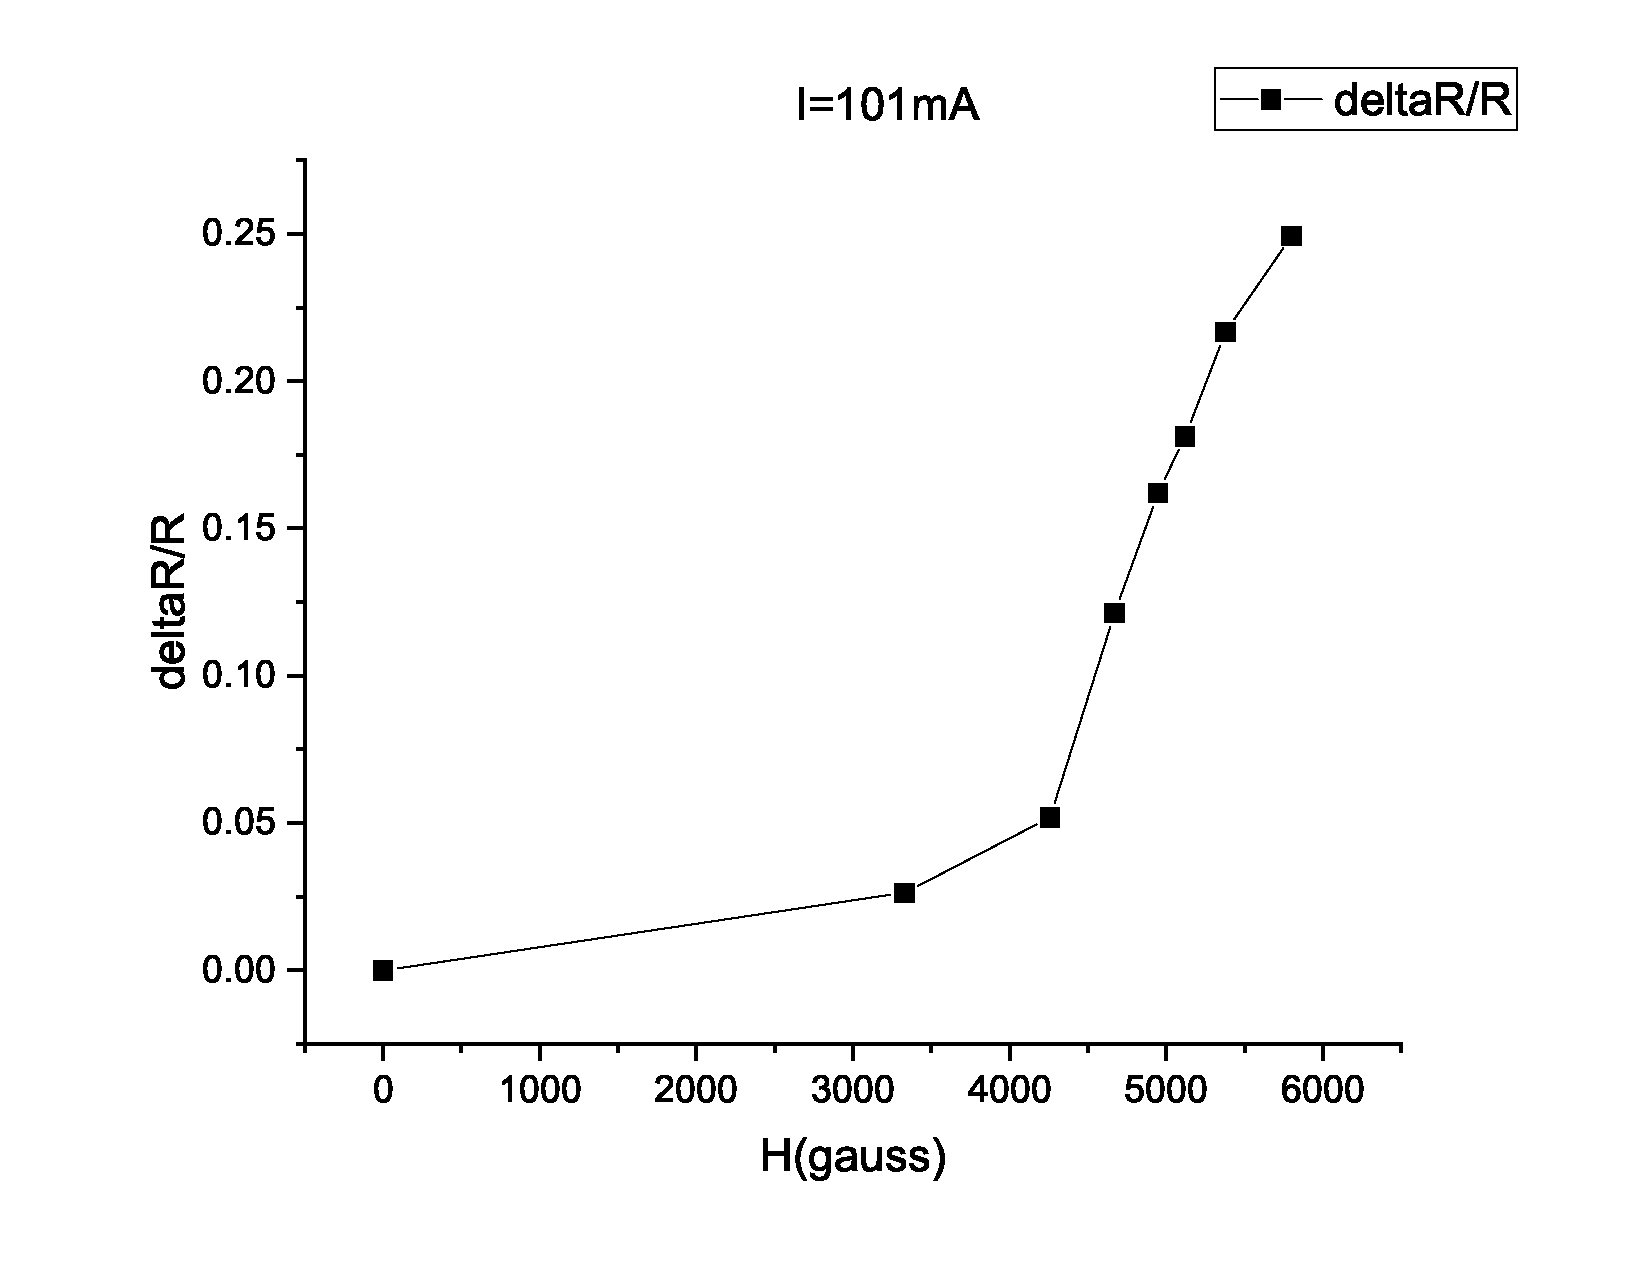
\includegraphics[width=0.95\columnwidth]{images/Graph3.eps}
                \caption{$\frac{\Delta R}{R}$ vs $H$}
                \label{fig:graph3}
            \end{figure}

            \begin{figure}[]
                \centering
                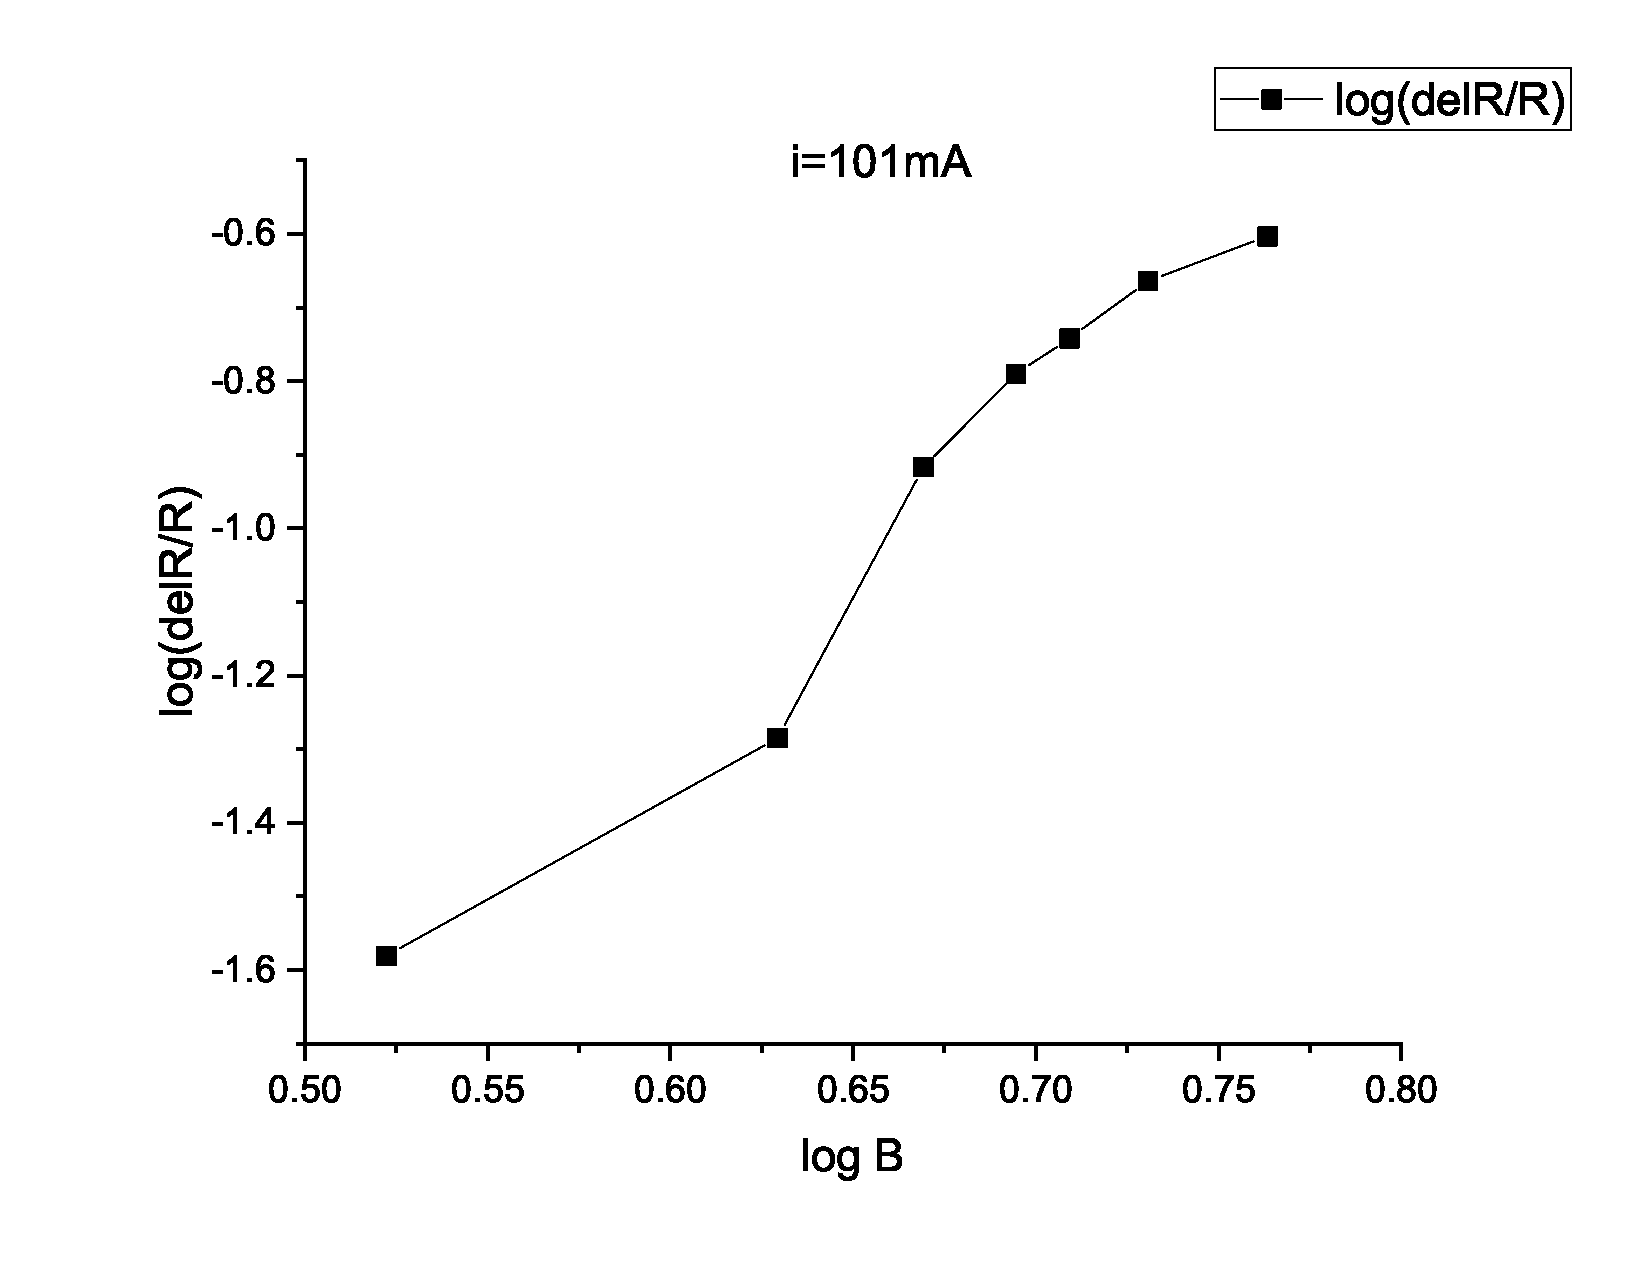
\includegraphics[width=0.95\columnwidth]{images/Graph4.eps}
                \caption{$\log(\frac{\Delta R}{R})$ vs $H$}
                \label{fig:graph4}
            \end{figure}

    \subsection{Hall effect}
        I=197.3mA

        Room temperature=$25^{\circ}C$ 
        
        Thickness(z)=0.5mm
        
        \begin{table}[]
	\centering
	\begin{tabular}{|l|l|}
	\hline
		H(gauss) & V(mV) \\ \hline
		2390 & -0.061 \\ \hline
		2540 & -0.062 \\ \hline
		3160 & -0.063 \\ \hline
		3480 & -0.064 \\ \hline
		4200 & -0.065 \\ \hline
		4500 & -0.066 \\ \hline
		4780 & -0.067 \\ \hline
		5200 & -0.068 \\ \hline
		5180 & -0.069 \\ \hline
	\end{tabular}
	\caption{Magnetoresistance Data for $I=101.0mA$}
	\label{tab:mag2}
\end{table}

        \begin{figure}[h!]
        \centering
        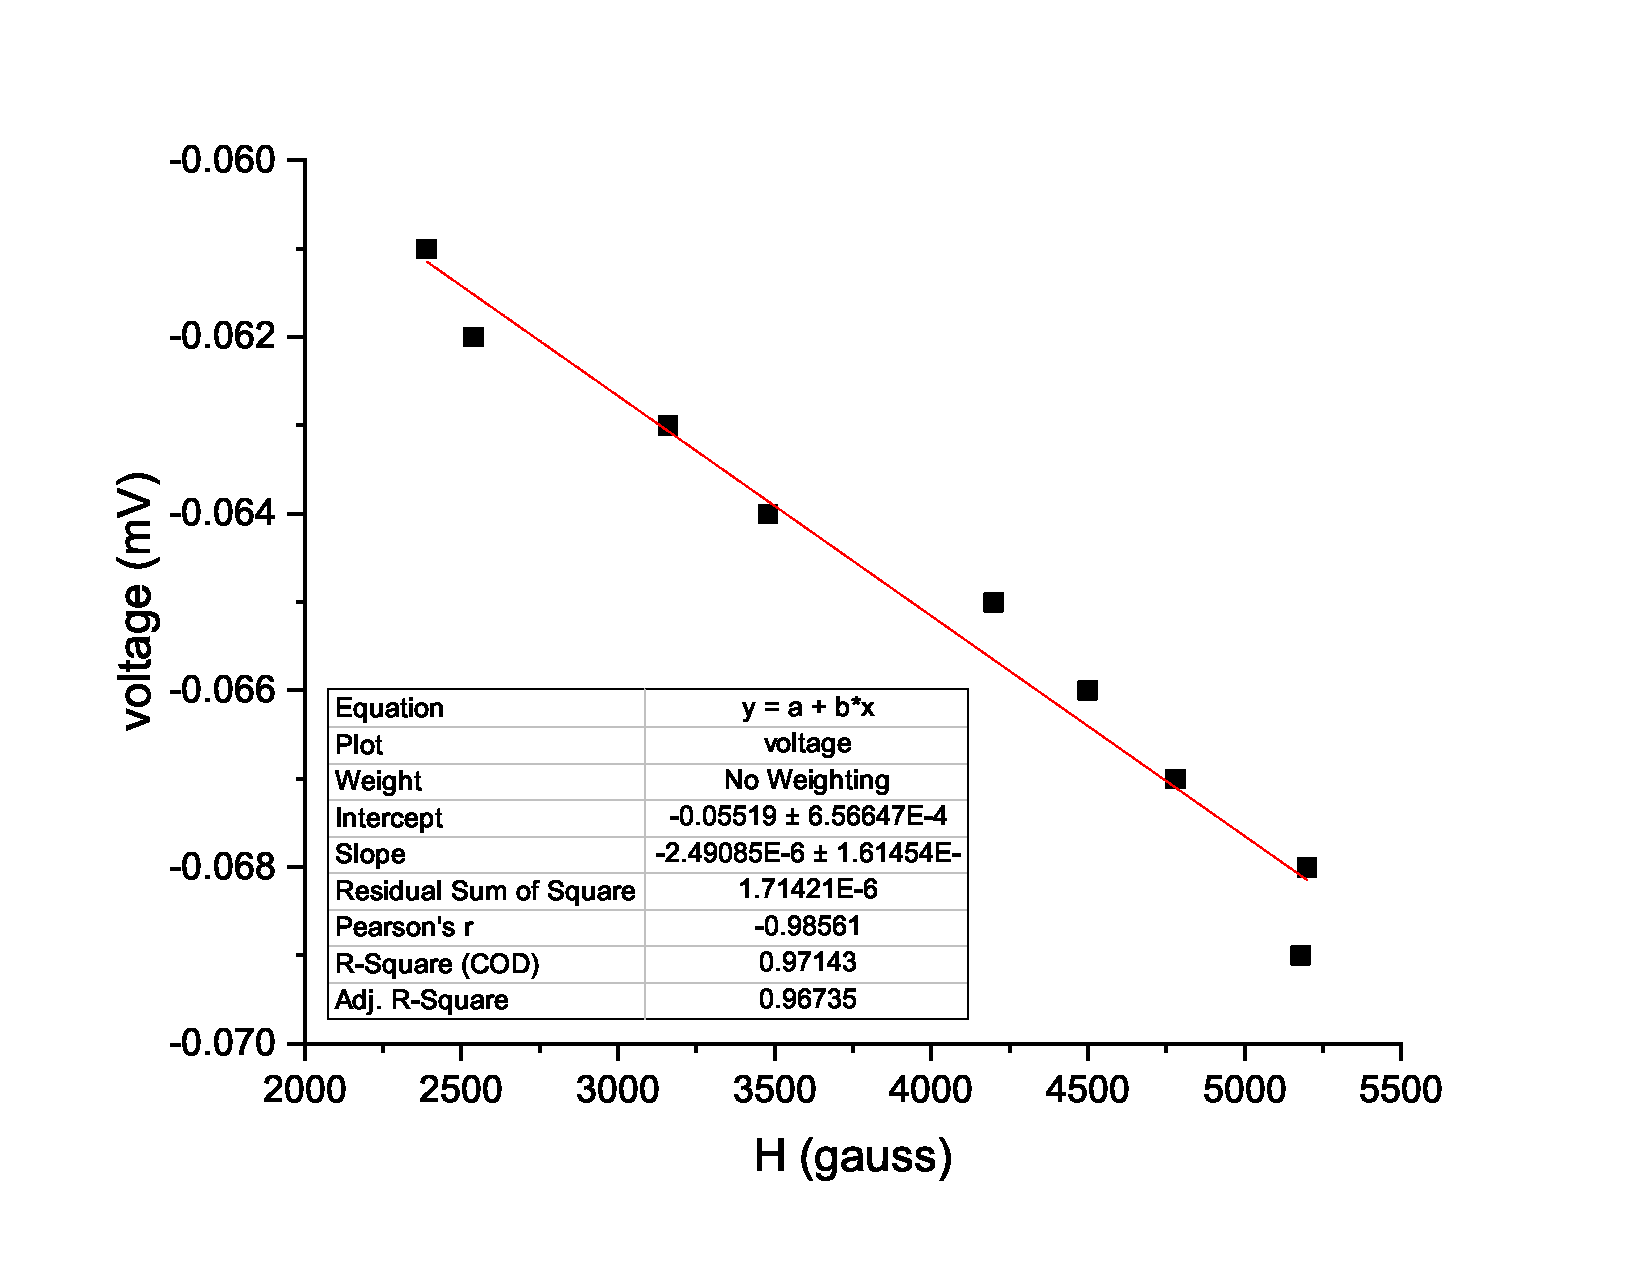
\includegraphics[width=0.95\columnwidth]{images/Graph6.eps}% Here is how to import EPS art
        \caption{\label{fig:epsart} hall voltage vs H}
        \end{figure}

        

        % from equation 2, we have\\
        % \(R=$$\frac{V_h z}{IH}$$\)\\
        % \(R=$$\frac{slope *z}{I}$$\) ,\\hall coefficient, 
        % R=-6.951 x 10^{-1}^2 ohm-cm /Gauss
        
        % \subsubsection{Error analysis}
        % we have, from equation 2, \\
        % \(($$\frac{\Delta R}{R}$$)^2=($$\frac{\Delta slope}{slope}$$)^2 + ($$\frac{\Delta I }{I}$$)^2\)\\
        % as z is error is not mentioned.
        % thus\\
        % \(\Delta R\)=+-0.45 x 10^-^1^2 ohm-cm/Gauss

    \subsection{Data analysis}
    We see that when the magnetic field strength increases, so does the magneto-resistance value. At low magnetic field intensities, the transition is gradual, but it speeds up as the strength rises. An increase in the Lorentz force on charge particles may be the cause. We can see that in the high magnetic field, Bismuth's resistance changes by 35 percent (i=198.5mA) and 25 percent (i=101mA). As the quantity of charge carriers diminishes, the change in magneto-resistance reduces along with it. Furthermore, as a result of a lack of charge carriers, we can see that the curve deviates from the predicted curve shape at low working current and saturates at high temperatures.

    We can see that there is a 6 percent inaccuracy in the value of the Hall coefficient. The next data point's variation could be the result of equipment heating up from prolonged usage and changes in the ambient temperature. The residual magnetic field in coils at zero current (3 Gauss) and variations in operational current may also be contributing factors. The charge density in metals is large as one could anticipate given that $R_h = 1$.